\paragraph{アーキテクチャ評価}
アーキテクチャ評価は、選んだ候補解が ASR を満たすかを確認し、手戻りが必要な箇所を見つける活動である。評価は最後に一度だけ行うものではない。分析と統合の途中で繰り返し行い、問題を早く見つけるほど、修正費用を抑えられる。

\begin{figure}[htbp]
\centering
\IfFileExists{swebok_structure/CH02.ソフトウェアアーキテクチャ(Software_Architecture)/2.3.ソフトウェアアーキテクチャ過程(Software_Architecture_Process)/2.3.2.アーキテクチャ設計(Architectural_Design)/2.3.2.3.アーキテクチャ評価(Architecture_Evaluation)/assets/fig-ch02-07.png}{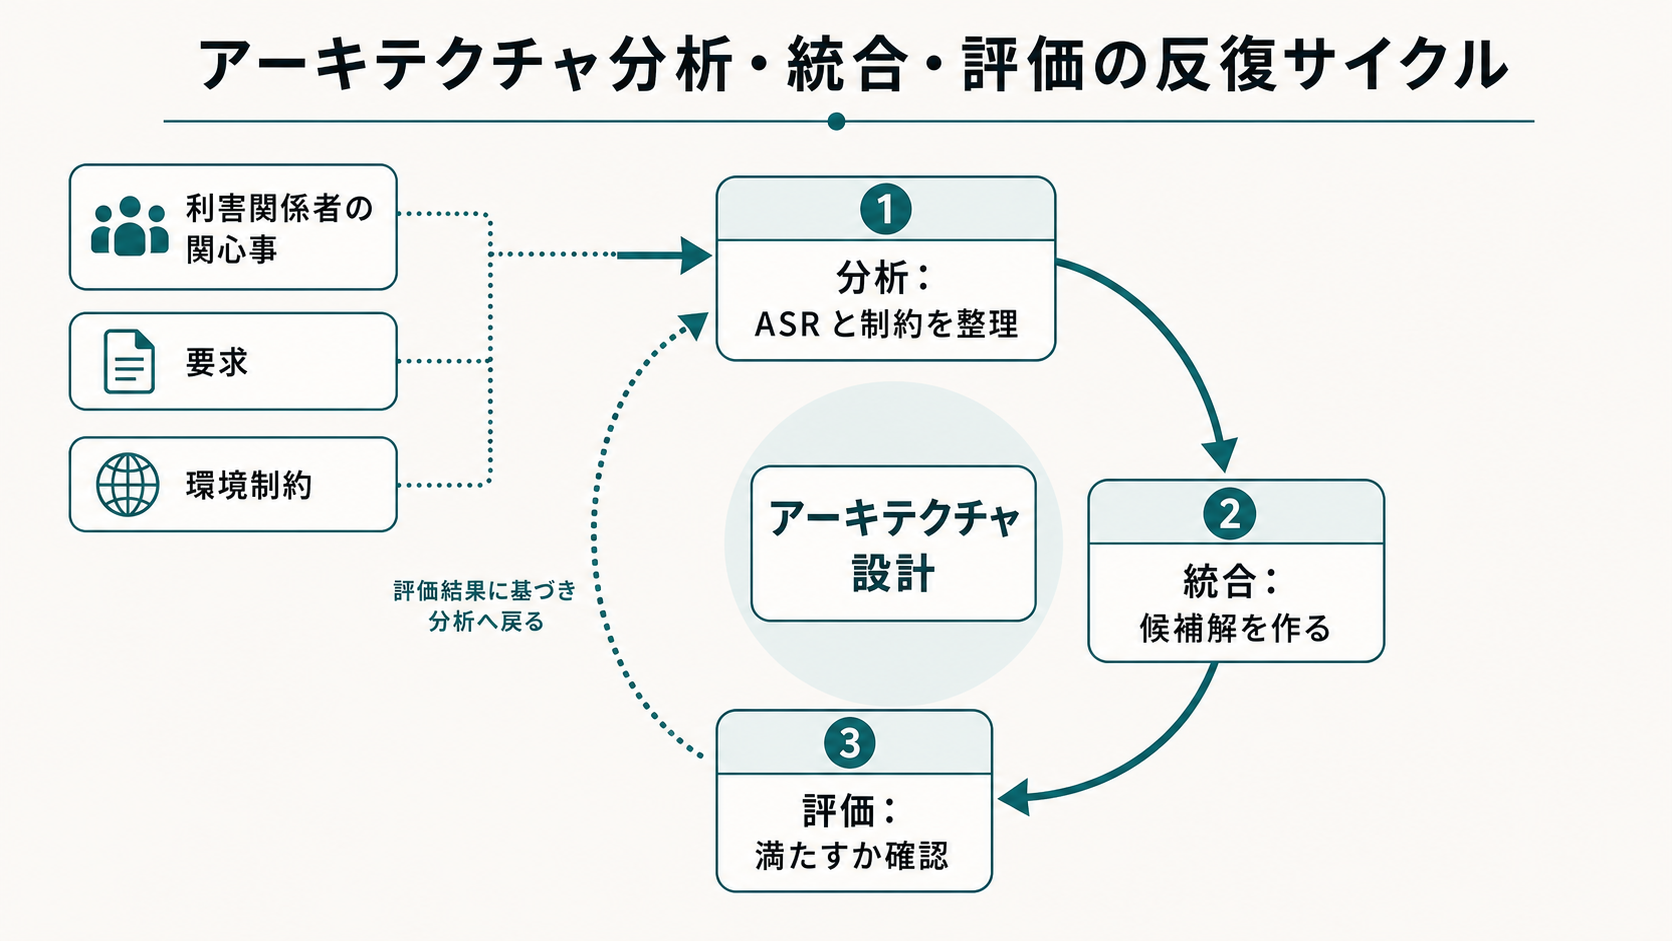
\includegraphics[width=0.96\linewidth]{swebok_structure/CH02.ソフトウェアアーキテクチャ(Software_Architecture)/2.3.ソフトウェアアーキテクチャ過程(Software_Architecture_Process)/2.3.2.アーキテクチャ設計(Architectural_Design)/2.3.2.3.アーキテクチャ評価(Architecture_Evaluation)/assets/fig-ch02-07.png}}{\fbox{\parbox[c][48mm][c]{0.9\linewidth}{\centering 画像生成待ち\\アーキテクチャ分析・統合・評価の反復サイクル}}}
\caption{アーキテクチャ分析・統合・評価の反復サイクル}
\label{fig:ch02-07}
\end{figure}
